\documentclass[12pt]{article}
\usepackage[utf8]{inputenc} %article book report letter
\usepackage{amssymb}
\usepackage{extarrows}
\usepackage{enumitem}
\usepackage{ctex}
\usepackage{amsthm}
\usepackage{amsmath}
\usepackage{framed}
\usepackage{amssymb}
\usepackage{geometry}

\usepackage{graphicx}
\usepackage[ruled,linesnumbered]{algorithm2e}
\usepackage{float}
\usepackage{booktabs}

%\usepackage[super]{gbt7714}
\usepackage{xcolor}
\usepackage{subcaption}
\usepackage{verbatim}
\usepackage{hyperref}
\usepackage{epstopdf}


\usepackage{cite}
%\usepackage{natbib}
%\setcitestyle{authoryear,round}

%\usepackage[numbers, sort&compress]{natbib}
\usepackage{gbt7714}
%\bibliographystyle{gbt7714-numerical}
%\usepackage[backend=biber,style=gb7714-2015ay]{biblatex}
%\usepackage[backend=biber,style=gb7714-2015ay,gbnoauthor=true]{biblatex}

\usepackage{hyperref}

\geometry{top=3cm,bottom=3cm}

\hypersetup{hidelinks,
	colorlinks=true,
	allcolors=black,
	pdfstartview=Fit,
	breaklinks=true
}

%\usepackage{listings,lstautogobble}

%\usepackage{listings} 
\usepackage{xcolor}

%\usepackage{minted}


\begin{document}
	\thispagestyle{empty}
	\begin{figure}[ht]
		\centering
		
\includegraphics[scale=0.56]{SYSULogo.pdf}
	\end{figure}
	
	\begin{center}
		\textbf{{\fontsize{35pt}{0pt}本科生毕业论文 (设计)}}
		
		\Large \textbf{{\fontsize{25pt}{0pt}Undergraduate Graduation Thesis (Design)}}
	\end{center}
	
	\begin{center}
		\huge 题目:\textbf{\underline{层叠成像中的相位恢复问题}}
		
	
	\end{center}
	
	\begin{quotation}
		\large \noindent
		院系 \\
		School(Department):\underline{~~~~~~~~~~~~~~~~~~数学学院~~~~~~~~~~~~~~~~~~~} \\
		专业 \\
		Major:\underline{~~~~~~~~~~~~~~~~~~~~~~~~~~~~~~~~数学与应用数学~~~~~~~~~~~~~~~~} \\
		学生姓名 \\
		Student Name:\underline{~~~~~~~~~~~~~~~~~~~~~~~~~~吴茼~~~~~~~~~~~~~~~~~~~~~~} \\
		学号 \\
		Student No:\underline{~~~~~~~~~~~~~~~~~~~~~~~~~~~~17307053~~~~~~~~~~~~~~~~~~~~~} \\
		指导教师(职称) \\
		Supervisor(Title):\underline{~~~~~~~~~~~~~~~~~李嘉 (副教授)~~~~~~~~~~~~~~~~~~~~~}
	\end{quotation}
	~\\
	\begin{center}
		时间:二零二二年四月十一日
		
		Date: April 11th 2022
	\end{center}
	
	\newpage
	\thispagestyle{empty}
	\begin{center}
		\Large  学术诚信声明
	\end{center}
	
	\begin{large}
	本人所呈交的毕业论文,是在导师的指导下,独立进行研究 工作所取得的成果,所有数据、图片资料均真实可靠。除文中已经注明引用的内容外,本论文不包含任何其他人或集体已经发表或撰写过的作品或成果。对本论文的研究作出重要贡献的个人和集体,均已在文中以明确的方式标明。本毕业论文的知识产权归属于培养单位。本人完全意识到本声明的法律结果由本人承担。\\ \\ \\
	$~~~~~~~~~~~$本人签名:$~~~~~~~~~~~~~~~~~~~~~~~~~~~~~~~$日期:
	\end{large}
	~\\ \\ \\
	\begin{center}
		\Large \textbf{Statement of Academic Integrity}
	\end{center}

	\begin{large}
	I hereby acknowledge that the thesis submitted is a product of my own independent research under the supervision of my supervisor, and that all the data, statistics, pictures and materials are reliable and trust- worthy, and that all the previous research and sources are appropriately marked in the thesis, and that the intellectual property of the thesis be- longs to the school. I am fully aware of the legal effect of this statement. \\ \\ \\
	$~~~~~~~~$Student Signature:$~~~~~~~~~~~~~~~~~~~~~~~~~~$Date:
	\end{large}
	\newpage
	\thispagestyle{empty}
	\begin{center}
		\LARGE \textbf{层叠成像中的相位恢复问题}
		
	
		%\LARGE \textbf{基于变量因子选择的中国 A 股市场量化交易研究}
	\end{center}
	\begin{center}
		\textbf{摘要}
	\end{center}
	
	%本文对中国A股市场量化交易进行分析,根据中国A股市场的股票定价因子对股价收益率进行预测。首先,在众多的定价因子进行选择,即特征选取和变量选取,目的是选择互相正交且重要的定价因子,对自变量进行降维,减少信息冗余,提高后续预测模型的训练精度;其次,将选取的特征作为输入,通过机器学习算法,比如常见的随机森林和神经网络等算法对下一期的股价进行预测;最后,根据预测的收益率,做多收益率最高的10\%的股票,做空收益率最低的10\%的股票,构造一个多空头寸的投资组合,对投资组合的收益率和夏普比率进行分析。
		本文主要讨论偏相干层叠成像中的相位恢复问题。 根据被偏向干效应污染的无相位的衍射图序列, 恢复出真实图像和用于成像的探针。 为了刻画偏向干效应,选用了多种物理模型中的一个,并详细讨论了它与一般化的多模态模型间的关系。 将直观的交替投影方法改进为ADMM算法,并拓展到多个模态的情形。 我们进行了三个仿真数值实验验证了算法的有效性。
		第一,模态逼近实验。 随着模态数目增加,逼近密度矩阵的精度提高,图像的恢复质量提升。算法恢复出来的模态与根据模型产生的标准答案高度相似。  第二,尝试在ADMM中加入正交化约束,避免搜索过程中不同模态的信息重叠,提升算法的效率。 第三, 有噪声的情形。 
	
	\textbf{关键词:相位恢复~  偏向干理论~ 层叠成像~ ADMM}
	
	\newpage
	\thispagestyle{empty}
	\begin{center}
		\large \textbf{Partially coherent ptychography} ~\\ ~\\
		\normalsize \textbf{Abstract}
		This paper mainly discusses the phase recovery in partially coherent ptychography. The real image and the probe are recovered from the phase-free diffraction pattern sequence contaminated by the partially coherent effect. To characterize this effect, a 'phobe vibration' model is chosen and its relationship to a generalized model is discussed in detail. The alternative projection method is improved to an ADMM algorithm and extended to the case of multiple modes.
		
		We conducted three numerical experiments to verify the effectiveness of the algorithm. First, approximation by the modes. As the number of modes increases, the accuracy of approximating the density matrix increases, and the quality of the recovered image improves. The modes recovered by the algorithm are highly similar to the standard answer generated from the model. Second, try to add orthogonalization constraints in ADMM to avoid redundant information of different modes in the searching process. Third, noisy case.
	\end{center}
	

	\textbf{Key words: Phase retrieval~  Coherence theory~ Ptychography~ ADMM}
	
	\newpage
	\thispagestyle{empty}
	\tableofcontents
	
	\newpage
	\thispagestyle{empty}
	\listoffigures
	
	\listoftables
	
	\newpage
	\setcounter{page}{1}
	\section{引言}
	
	\subsection{选题背景与意义}

	
	层叠成像(Ptychography)是科学领域中一种流行的成像技术,如凝聚态物理、细胞生物学、材料科学和电子学等。 它通过处理从感兴趣对象散射的许多相干干涉图案来生成图像。 层叠成像可用于可见光、X 射线、极紫外 (EUV) 或电子。与传统的镜头成像不同,层叠成像不受镜头引起的像差等影响,这对于原子级波长成像尤其重要,因为在这种情况下,制造满足要求的镜头既困难又昂贵。 因此,层叠成像在高分辨重建上具有优势,能用于探测极为细微的结构。
	
	该技术的另一个重要优点是它可以非常清楚地看到透明物体。这是因为它对穿过样品的辐射的相位敏感,因此它不依赖于吸收辐射的物体。在可见光生物显微镜的情况下,这意味着不需要对细胞进行染色或标记来产生对比度。
	
	在相干光层叠成像实验中,根据实验设备事先确定的扫描位置,局部的相干X射线探头扫描样本,而探测器在远场收集一系列观测数据。 由于现有的接收器往往只对光的强度敏感,所以衍射图像中的相位会丢失,信息的丢失对图像的重建造成了挑战。 我们的目标是从强度测量序列中获得样本的高分辨率重建, 而这往往依赖于迭代的相位恢复算法。 %figure
	
在物理学里,相干性(coherence)描述波与自己、波与其它波之间对于某种内秉物理量的相关性质。 当两个波彼此相互干涉时,因为相位的差异,会造成相长干涉或相消干涉。假若两个正弦波的相位差为常数,则这两个波的频率必定相同,称这两个波“完全相干”(coherent)。两个“完全不相干”的波,例如白炽灯或太阳所发射出的光波,由于产生的干涉图样不稳定,无法被明显地观察到。在这两种极端之间,存在着“部分相干”(partially coherent)的波。 在成像实验中,往往需要用到完全相干的光源。产生完全相干的光源需要苛刻的实验条件,有时候光源实际上是部分相干的,这就会对成像的结果造成影响。 对光源苛刻的要求,成为层叠成像发展中的一大限制因素。 相干层叠成像实验通常依靠光圈来定义相干照明。为了提高光源相干性,世界各地的研究机构都在投入大量资源来生产更亮的 X 射线源。同时,大多数产生的 X 射线光子目前都被二级孔径丢弃,这会造成大量浪费。即使有足够强度的相干光,曝光期间所需的稳定性通常也是另一个限制因素。因此,研究者们开始思考,是否能在较放松的实验条件,即偏相干光源下,建立图像重建的方法,以减少光强和稳定性限制。
	

	
	
	

	\subsection{国内外研究现状和相关工作}
		起初,为了重建图像,物理学家首先开始研究相位恢复问题。 自从综述文章\cite{all}将这个问题引入应用数学界,数学家提出了许多新的计算方法。 比如,在纯相干情形,作者将传统的AP改进为ADMM算法(Alternating Direction Method Of Multipliers),提高了算法稳定性和效率\cite{admm}。然而,偏相干成像被讨论得较少。
	
		为了表示偏相干效应,研究者们提出了不同的前向模型。物理学家在 \cite{theory} 中提出了一个通用模型,它是一种基于quantum state tomography\cite{quan}的盲层叠成像模型。 它假设探针处于具有$r$个模态的混合状态。在\cite{mix}中,研究者根据这个模型设计了算法,并进行了数值实验。诸如AP(Alternative Projection,交替投影)之类的算法可以从相干情况扩展到偏相干情况以找到$r$个主要模态。 这个通用模型现在成为偏相干层叠成像中的主流模型. 尽管该模型在各种情况下成功地重建了图像,例如具有平移模糊的“飞行扫描”数据,但多种模态的物理解释尚不清楚,并且与相干函数的关系是间接的。
		
		因此,研究者们对不同的实验设置提出了一些特定的模型\cite{psf}。 在一个较简单的模型中\cite{direct},偏向干效应被解释为接收器上多个像素的合并,这体现为对观测强度数据加上了一个卷积模糊。在 \cite{chang} 中,作者提出了一个较新的模型,将偏相干效应描述为振动核 $ \kappa $ 在主要模态 $\omega$ 上的模糊。因为这个前向模型很难计算,他们使用了GDP(Gradient Decomposition of the Probe, 探针梯度分解),一种新的前向模型,来近似它。然后他们提出了 GDP-ADMM,这是一种迭代求解器,可以联合优化图像、探针和模糊核函数的方差。然而,当模糊核方差大小增加时,逼近精度下降,结果看起来很模糊。他们假设内核是高斯的,只优化方差参数,这可能不适合真实世界的数据。
	
	在本文中,我们想用数学语言来描述偏相干,并设计一种有效的算法来解决这个问题。我们将关注\cite{chang}中的振动模型,先通过数学推导揭示它于通用模型 \cite{mix}之间的联系,在通用模型的框架下求解,目标是找到$r$个而不是单一的模态。 比起\cite{mix}中的多模态AP, 我们将\cite{chang}中纯相干情形的ADMM算法推广到偏相干的情形, 并加入正交约束辅助模态的搜素。 我们进行了仿真实验,展示恢复的图像和模态,验证了算法的有效性。
	%为了从理论上证明模型和算法的合理性,需要在合适的探针 $\omega$和振动核$\kappa$假设下,对模型的逼近误差和算法的收敛速度进行定量分析。
	
	\subsection{本文论文结构与章节安排}
	本文共分为五节,每章节的内容如下:
	
	第一节:引言。介绍了层叠成像技术的优势和应用,纯相干层叠成像的限制,从而提出偏相干层叠成像的研究背景和意义。 然后介绍了偏相干层叠成像在模型、算法方面的研究现状和相关工作
	
	第二节:模型。介绍偏相干效应的不同模型,包括了多模态通用模型和两个特殊模型,并阐述他们的联系。
	
	第三节:算法。 介绍带正交约束的ADMM算法,用于求解偏相干层叠成像的多模态通用模型。 明确写出每个子问题的更新步骤,一些推导被放入附录中。
	
	第四节:实验。 首先介绍了实验中的参数设置, 衡量算法效果的度量指标。然后介绍了实验中对模态进行操作的一些子算法,包括:初始化,正交化和压缩。进行了三个数值实验和结果展示:多模态逼近实验,正交约束实验和噪声实验
	
	第五节:总结和展望。 
	


	\newpage
\section{模型}

在本节中,我们从纯相干模型引入,再介绍通用的偏相干模型和两个特殊的偏向干模型。 最后,我们阐述模型之间的联系,指出我们的目标模型也可以放在通用偏向干模型下求解。

\subsection{纯相干模型}


在离散的情况下, $u \in \mathbb{C}^{n}$ 是一个2D图像, 有着 $\sqrt{n} \times \sqrt{n}$ 个像素, $\omega \in \mathbb{C}^{\bar{m}}$ 是一个2D的局部探针, 有着 $\sqrt{\bar{m}} \times \sqrt{\bar{m}}$ 个像素.

$f_{j} \in \mathbb{R}_{+}^{\bar{m}}(\forall 0 \leq j \leq N-1)$ 是一叠没有相位的观测值. 这里 $|\cdot|$ 代表 一个向量逐个元素取绝对值, o 代表逐个元素的乘法,  $\mathcal{F}$ 代表标准化后的离散二维傅里叶变换. 每个 $\mathcal{S}_{j} \in \mathbb{R}^{\bar{m} \times n}$ 是一个 0-1 矩阵, 将大小为 $\bar{m}$ 的区域 $j$ 从 图像 $u$ 中割下来.

\begin{equation}
\label{basic}
f_{j}=\left|\mathcal{F}\left( \mathcal{S}_{j} u  \circ \omega \right)\right|^{2} 
\end{equation}

在实际中,由于无法完全了解该探针,我们需要解决盲层叠成像的相位恢复 (BP-PR) 问题:
%In practice, as the probe is almost never completely known, one has to solve a blind ptychographic phase retrieval (BP-PR) problem:

Find $\omega \in \mathbb{C}^{\bar{m}}$ and $u \in \mathbb{C}^{n}$ s.t. $|\mathcal{A}(\omega, u)|=\boldsymbol{a}$,

在这里 双线性 算子 $\mathcal{A}: \mathbb{C}^{\bar{m}} \times \mathbb{C}^{n} \rightarrow \mathbb{C}^{m}$ 和 $\mathcal{A}_{j}: \mathbb{C}^{\bar{m}} \times \mathbb{C}^{n} \rightarrow \mathbb{C}^{\bar{m}} \forall 0 \leq j \leq N-1$ 的意义如下:

$\mathcal{A}(\omega, u):=\left(\mathcal{A}_{0}^{T}(\omega, u), \mathcal{A}_{1}^{T}(\omega, u), \ldots, \mathcal{A}_{N-1}^{T}(\omega, u)\right)^{T}$, $\mathcal{A}_{j}(\omega, u):=\mathcal{F}\left(\omega \circ \mathcal{S}_{j} u\right)$

和 $\boldsymbol{a}:=\left(\boldsymbol{a}_{0}^{T}, \boldsymbol{a}_{1}^{T}, \ldots, \boldsymbol{a}_{N-1}^{T}\right)^{T} \in \mathbb{R}_{+}^{m}$.

\subsection{两个具体的偏相干模型}
\label{section:specific models}
当光源不是纯相干时,成像可能被偏向干效应污染。 在不同的物理背景下,研究者提出不同的模型刻画偏向干效应。 本小节中,我们首先介绍我们目标求解的模型。 然后再介绍一个密切相关而且更简单的模型。

\subsubsection{模型一: 目标模型\cite{chang}}
我们的目标模型中,偏相干效应被表示为成像探针$\omega$的振动。 在连续情形:
\begin{equation}
f_{p c, j}(q) = \int\left|\mathcal{F}_{x \rightarrow q}\left(\mathcal{S}_{j} u(x) \omega(x-y)\right)\right|^{2} \kappa(y) \mathrm{dy} 
\end{equation}

这里 $f_{p c}$ 偏向干情形下的观测强度, $\mathcal{F}_{x \rightarrow q}$ 是标准傅里叶变换。 $\kappa$ 是一个在0处突起的函数, 如高斯函数. 设置 $\kappa$ 为狄拉克函数 将它化简为纯相干模型 (\ref{basic}).

在离散情形下:
\begin{equation}
f_{p c, j}=\sum_{i} \kappa_{i}\left|\mathcal{F}\left( \mathcal{S}_{j} u \circ \left(\mathcal{T}_{i} \omega\right) \right)\right|^{2}
\label{model:target}
\end{equation}


符号的含义解释如下: 平移算子 $\mathcal{T}_{i}$, 离散高斯函数的权重 $\left\{\kappa_{i}\right\}$, 探针设为周期性边界条件.

广泛地说, 解决 (\ref{model:target})是一个非线性病态反问题, 我们不知道的有模糊核 $\kappa$, 探针$\omega$, 和目标图像$u$. 
%\textbf{And it is the main target in this research.}



\subsubsection{模型二\cite{psf}}
在这个更简单的模型中,偏相干效应被刻画为探测器上的卷积模糊。

\begin{equation}
\label{simple}
f_{p c}=f * \kappa
\end{equation}

这里 $f_{p c}$ 是观测到的偏向干强度, $f$ 是纯相干情形下观测到的强度 (\ref{basic}), $*$ 是卷积算子,  $\kappa$ 是未知的模糊核函数 



我们注意到 (\ref{model:target}) 与
(\ref{simple})不同 ,因为 (\ref{model:target}) 说明了探针振动的模糊效果,而 (\ref{simple}) 可以解释为探测器模糊或合并多个像素。

\subsection{通用分解模型}
这部分介绍了物理学家提出的通用偏相干模型\cite{mix}。 它是基于quantum state tomography\footnote{\url{https://homepage.univie.ac.at/reinhold.bertlmann/pdfs/T2_Skript_Ch_9corr.pdf}定理9.1的盲ptychography模型。 这里包含了许多量子力学中的符号。}。 假设 探针 $w$ 处于混合状态以表示偏向干的效果。


\subsubsection{模型描述}

通用分解模型是求解偏向干效应的主流模型,它刻画偏向干效应的方式是将纯相干情形的一个模态$\omega$拓展为$r$个模态。 

\begin{equation}
\label{sep} 
\begin{aligned}
&\mbox{Find } u, r \mbox{ othogonal $w_k$   }s.t. \\
&f_{p c, j}=\sum_{k=1}^r \left|\mathcal{F}\left( \mathcal{S}_{j} u \circ \left(\omega_k\right) \right)\right|^{2} (0\leq j \leq N-1)
\end{aligned}
\end{equation}




%Denote $O_j \in C^{\bar{m} \times \bar{m}}$ as a (diagonal) matrix to represent linear transform to $w$, s.t. $\mathcal{S}_{j} u \circ \omega = O_j w$. Denote $f_q^* \in C^{1 \times \bar{m}}$ as a row vector  constructed from Fourier transform $\mathcal{F}$, to represent projection on frepuency element. Construct measurement matrix $ \mathcal{I}_{j \mathbf{q}} = O_j^*f_qf_q^*O_j$ and density matrix $\rho$, we get another form(actually a natural one in quantum state tomography) of the model:
将 $O_j \in C^{\bar{m} \times \bar{m}}$ 表示为(对角线)矩阵,以表示对 $w$ 的线性变换,s.t. $\mathcal{S}_{j} u \circ \omega = O_j w$。 将 $f_q^* \in C^{1 \times \bar{m}}$ 表示为由傅里叶变换 $\mathcal{F}$ 构造的行向量,以表示在频率元素上的投影。 构造测量矩阵$ \mathcal{I}_{j \mathbf{q}} = O_j^*f_qf_q^*O_j$ 和密度矩阵$\rho$,我们得到另一种形式(实际上是quantum state tomography中的自然形式):

\begin{equation}
\label{lift}
\begin{aligned}
&\mbox{Find } u,\rho,s.t.\\
&f_{pc,j}(q) = Tr(\mathcal{I}_{j \mathbf{q}} \rho ) (0\leq j \leq N-1)\\
&\rho \mbox{ is positive semi-definite, with rank}\leq r 
\end{aligned}
\end{equation}

接下来,我们将解释这种形式的推导。

简单的计算过程:
$$
f_{pc,j}(q) = |f_q^*O_j w|^2 = (f_q^*O_j w)^*(f_q^*O_j w) = w^*(O_j^*f_qf_q^*O_j)w
$$
$$
=Tr[w^*(O_j^*f_qf_q^*O_j)w]=Tr[(O_j^*f_qf_q^*O_j) (ww^*)]
$$
$$
=Tr(  \mathcal{I}_{j \mathbf{q}} \rho )
$$





这有点像相位提升的过程。



当$w$ 处于单一状态(希尔伯特空间中的一个向量)时,$\rho=w^*w$ 是一个秩一矩阵。 在偏相干的情况下,我们使用混合状态来建模 $w$。 例如,在状态 $\psi_1$ 中的概率为 0.5,在 $\psi_2$ 中的概率为 0.5($\psi_1$ 和 $\psi_2$ 在这里不一定是正交的)。 现在$w$不能再用向量来表示了(ps.$w \neq p_1\psi_1 + p_2 \psi_2$,后者仍然是一个确定的纯状态向量)。 取而代之地是,密度矩阵泛化为具有更高秩的矩阵,用以表示混合状态:
$$
\rho = \sum_k p_k \psi_k \psi_k^*
$$



容易发现$\rho$是一个半正定矩阵,我们可以利用谱定理分解$\rho$,得到$r$(rank of $\rho$)个主要的正交模态$w_k$:
\begin{equation}
\label{ort}
\rho = \sum_{k=1}^{r} w_k w_k^*
\end{equation}



$$
f_{pc,j}(q) = \operatorname{Tr} \mathcal{I}_{j \mathbf{q}} \rho
= \operatorname{Tr}[ \mathcal{I}_{j \mathbf{q}}  \sum_{k=1}^{r} w_k w_k^*]
$$
$$
=
\sum_{k=1}^r w_k^*\mathcal{I}_{j \mathbf{q}} w_k 
=
\sum_{k=1}^r |f_q^*O_j w_k|^2 
$$
而这正是 \eqref{sep}$
f_{pc,j}=\sum_{k=1}^r \left|\mathcal{F}\left( \mathcal{S}_{j} u \circ \left(\omega_k\right) \right)\right|^{2}  
$. ($f_{pc,j}(q)$ 是在频率 $q$ 处的单一值,而 $f_{pc,j}$ 是整个衍射图像)

我们也可以把这个写成二次型的形式:
\begin{equation}
\label{quadratic}
\begin{aligned}
f_{pc,j}(q) &=  \operatorname{Tr} \mathcal{I}_{j \mathbf{q}} \rho =Tr[(O_j^*f_qf_q^*O_j)\rho]
= Tr[(O_j^*f_q)^*\rho (O_j^*f_q)] = (O_j^*f_q)^*\rho (O_j^*f_q) \\
&= g_q^* \rho g_q = \sum_{x_1} \sum _{x_2}  \overline{g_q(x_1)} \rho(x_1,x_2) g_q(x_2)
\end{aligned}
\end{equation}

where $g_q = O_j^*f_q =  \overline{S_ju} \circ f_q$, $\overline{g_q} = S_ju \circ \overline{f_q}$

这是  \cite{psf}中提到模型的离散版本.  

\subsubsection{模型之间的关系}
\label{section:reference}
在本小节中,我们将解释通用模型如何与特定模型 \eqref{model:target} 和 \eqref{simple} 联系。

对于 \eqref{simple}, 我们介绍 coherence function 的定义:
$$
\gamma(x_1,x_2) = \dfrac{\rho(x_1,x_2)}{w(x_1) \overline{w(x_2)} }
$$
也就是:
\begin{equation}
\gamma = \rho ./ ( w w^*), \rho = \gamma \circ (ww^*) \label{eq: coherence}
\end{equation}


这里 $./$ 意味着 逐个元素的除法.

当我假设 coherence function$\gamma\left(\mathbf{x}_{1}, \mathbf{x}_{2}\right)$ 只与两个点之间的距离有关 $\mathbf{x}_{1}, \mathbf{x}_{2}$, i.e. $\gamma\left(\mathbf{x}_{1}, \mathbf{x}_{2}\right)=\gamma\left(0, \mathbf{x}_{2}-\mathbf{x}_{1}\right)$, 我们可以把远场强度写成一个卷积的形式\cite{psf}$f_{pc} = \kappa * f $. 

如果我们知道PSF(point spread function) $\kappa(q)$, 那我们可以得到它的傅里叶逆变换 $\gamma(0,x) = (\mathcal{F}^{-1}\kappa)(x)$. 在这个假设上,我们得到 $\gamma(x_1,x_2)$.  如果我们也知道探针 $w$, 那我们可以得到 $\rho$, SVD 帮助我们找到主要模态 $w_k$。


最后我们考虑目标模型 \eqref{model:target},这里有两种看法。 第一种是直接从时间域上看,我们把 $\kappa_{i}$ 放在里面:
\begin{equation}
f_{p c, j}=\sum_{i} \left|\mathcal{F}\left( \mathcal{S}_{j} u \circ \left( \sqrt{\kappa_{i}}\mathcal{T}_{i} \omega\right) \right)\right|^{2}
=
\sum_{i} \left|\mathcal{F}\left( \mathcal{S}_{j} u \circ \left( \hat{\omega}_i\right) \right)\right|^{2}
\label{model:gradient decomposition}
\end{equation}
%Multiple modes $\hat{w}_i$ are produced by shifted $w$. Then we can construct density matrix and use truncated SVD to get a low-rank approximation. 

多种模态 $\hat{w}_i$ 由移位 $w$ 产生。 然后我们可以构造密度矩阵并使用SVD 得到一个低秩近似。
$$
\rho = \sum_i \hat{w}_i \hat{w}_i^* \approx \sum_{k=1}^{r} w_k w_k^* 
$$

第二种是从频率域上看:

  \begin{equation}
\begin{aligned}
f_{p c, j}(q) &= \int\left|\mathcal{F}_{x \rightarrow q}\left(\mathcal{S}_{j} u(x) \omega(x-y)\right)\right|^{2} \kappa(y) \mathrm{d} y\\
&= \int \mathcal{F}_{x \rightarrow q}\left(\mathcal{S}_{j} u(x) \omega(x-y)\right) \overline{ \mathcal{F}_{x \rightarrow q}\left(\mathcal{S}_{j} u(x) \omega(x-y)\right) }  \kappa(y)     dy\\
&= \int \int \mathcal{S}_{j} u(x_1) \omega(x_1-y) e^{-iqx_1} dx_1 \overline{ \int \mathcal{S}_{j} u(x_2) \omega(x_2-y) e^{-iqx_2}dx_2 }  \kappa(y)   dy \\
&= \int \int \mathcal{S}_{j} u(x_1)e^{-iqx_1} \omega(x_1-y)  dx_1 \overline{ \int \mathcal{S}_{j} u(x_2)e^{-iqx_2} \omega(x_2-y) dx_2 }  \kappa(y)   dy\\
&= \int \int \widehat{\mathcal{S}_{j} u(x_1)e^{-iqx_1}} \widehat{\omega(x_1-y)}  dx_1' \overline{ \int \widehat{(\mathcal{S}_{j}u)(x_2) e^{-iqx_2} }  \widehat{\omega(x_2-y)} dx_2' } \kappa(y)   dy\\
& = \int\int  
\widehat{\mathcal{S}_{j} u(x_1)e^{-iqx_1}} \widehat{\omega}(x_1')e^{-iyx_1'}  \overline{ \widehat{\mathcal{S}_{j} u(x_2)e^{-iqx_2}} \widehat{\omega}(x_2')e^{-iyx_2'} }   \int   \kappa(y)   dy
dx_1' dx_2' \\
& =  \int\int  
\widehat{(\mathcal{S}_{j}u)}(x_1' + q) \widehat{\omega}(x_1')   \overline{ \widehat{(\mathcal{S}_{j}u)}(x_2' + q) \widehat{\omega}(x_2') }   (\int   \kappa(y)e^{-iy(x_1'-x_2')}  dy ) \\
& = \int\int  
\widehat{(\mathcal{S}_{j}u)}(x_1' + q) \widehat{\omega}(x_1')   \overline{ \widehat{(\mathcal{S}_{j}u)}(x_2' + q) \widehat{\omega}(x_2') }    \hat{\kappa}(x_1'-x_2')  
dx_1' dx_2'
\end{aligned}
\end{equation}
然后我们可以得到频域上的密度矩阵:
$$
\hat{\rho}(x_1',x_2') =  \hat{\omega}(x_1') \overline{\hat{\omega}(x_2')}
\hat{\kappa}(x_1'- x_2')
$$
$$
\hat{\rho}  =\hat{\kappa} \circ (\hat{\omega}\hat{\omega}^*) 
$$
注意到这和之前的 \eqref{eq: coherence}很像, 上面的$\gamma$相当于这里的$\hat{\kappa}$,只是前者在时间域,后者在频率域. 二者的密度矩阵,都是由一个卷积核$\kappa$生成的toeplitz结构的矩阵,和一个由主要模态$\omega$生成的秩一矩阵,两个矩阵逐个元素相乘的结果。 这样生成的密度矩阵结合了$\omega$和$\kappa$的结构,往往具有很好的近似低秩性质,这为我们使用通用模型去寻找$r$个主要模态以近似密度矩阵提供了理论保证。



通过上面的不同模型间的联系,我们可以得到“标准模态分解”作为数值实验的参考。 总的来说,两个特殊模型的密度矩阵结构相似, 二者密切相关。 它们都可以被放到通用模型的框架下解释和求解。


	
	\newpage
\section{基于ADMM的数值算法}

本节将从通用模型入手,设计基于ADMM的数值算法。

常用的AP可以被重写成ADMM形式, 它更快而且更稳定. 我们推广 \cite{admm} 中的ADMM算法到多模态的情形. 为了引导算法减少多个模态之间的信息冗余,提高搜素效率,我们还引入了模态间的正交约束。

现在$w \in \mathbb{C}^{(px\times py) \times r}$ 是r个模态$r$ . $u \in \mathbb{C}^{Nx\times Ny}$ 是图像.  $f \in \mathbb{C}^{(px \times py) \times N}$ 是真实观察到的衍射图像. 记 $Y=\sqrt{f}$ 为对应模长 .

一个辅助变量 $z=\mathcal{A}(\omega, u) \in \mathbb{C}^{(px \times py) \times N \times r}$ 被引入. $\mathcal{A}$ 是一个从图像 $u$ 和$r$个不同模态$w_k:=w(:,:,k) \in \mathbb{C}^{px \times py}$ 产生衍射图像序列的算子,每个模态产生$N$ 帧. 对于多维向量,符号 : 表示自由维度,我们可以固定一些索引来从原始向量中提取特定维度。  

根据通用模型\ref{model:target}, 问题叙述为:
$$
\begin{aligned}
&\mbox{Find } \omega,u \ s.t.\\
& \bar{\mathcal{A}}(\omega, u)=Y\\
\end{aligned}
$$


这里 $\mathcal{A}: \mathbb{C}^{(px\times py)\times r} \times \mathbb{C}^{Nx \times Ny} \rightarrow \mathbb{c}^{(px \times py) \times N \times r}$,$\mathcal{A}_{j}: \mathbb{C}^{px\times py} \times \mathbb{C}^{Nx \times Ny} \rightarrow \mathbb{C}^{px\times py} $,
$\bar{\mathcal{A}_j}:\mathbb{C}^{(px\times py)\times r} \times \mathbb{C}^{Nx \times Ny} \rightarrow \mathbb{R}_+^{(px \times py)}$, 而且 $\bar{\mathcal{A}}:\mathbb{C}^{(px\times py)\times r} \times \mathbb{C}^{Nx \times Ny} \rightarrow \mathbb{R}_+^{(px \times py) \times r} (\forall 0 \leq j \leq N-1)$ 被表示为:

$z(:,:,j,k) = \mathcal{A}_{j}(\omega_k, u):=\mathcal{F}\left(\omega_k \circ \mathcal{S}_{j} u\right) \in \mathbb{C}^{px\times py}$,

$z(:,:,:,k) =\left(\mathcal{A}_{0}^{T}(\omega_k, u), \mathcal{A}_{1}^{T}(\omega_k, u), \ldots, \mathcal{A}_{N-1}^{T}(\omega_k, u)\right)^{T} 
\in \mathbb{C}^{(px\times py) \times N}$,

$z(:,:,j,:) =\left(\mathcal{A}_{j}^{T}(\omega_1, u), \mathcal{A}_{j}^{T}(\omega_2, u), \ldots, \mathcal{A}_{j}^{T}(\omega_r, u)\right)^{T} 
\in \mathbb{C}^{(px\times py) \times r}$.


,

$\bar{\mathcal{A}}_{j}(\omega, u):= \sum_{k=1}^r |\mathcal{A}_{j}(\omega_k, u)|^2 \in \mathbb{R}_+^{px\times py}$,

$\bar{\mathcal{A}}(\omega, u):=\left(\bar{\mathcal{A}}_{0}^{T}(\omega, u), \bar{\mathcal{A}}_{1}^{T}(\omega, u), \ldots,\bar{\mathcal{A}}_{N-1}^{T}(\omega, u)\right)^{T} 
\in \mathbb{R}_+^{(px\times py) \times N}$,



和 $Y=\left(\boldsymbol{a}_{0}^{T}, \boldsymbol{a}_{1}^{T}, \ldots, \boldsymbol{a}_{N-1}^{T}\right)^{T} \in \mathbb{R}_{+}^{(px \times py) \times N }$.




$\mathcal{G}(z)= || \sqrt{ \sum_{k=1}^{r} |z(:,:,:,k)|^2} - Y||^2$ 测量模型计算的值与真实值之间的差异。\\
$\mathcal{X}_{1}$ 和 $\mathcal{X}_{2}$ 表示$w$ 和 $u$ 的先验范围. $l=px \times py$, $\mathcal{X}_{3}$ 是正交指示函数 $D\alpha \in \mathbb{C}^{l \times r}$ ( $D \in  \mathbb{C}^{l \times r}$标准正交 s.t. $D^*D=I$),  $\alpha \in  \mathbb{R}^{r \times r}$表示模长.
$\Omega$ 是一个形状调整算子, $\Omega(D\alpha) := reshape(D\alpha,[px,py,r]) \in \mathbb{C}^{(px \times py) \times r}$. 有时候我们将 $\Omega(D^k\alpha^k)$ 简写为 $\Omega^k$ , $\Omega(D\alpha)$ 简写为 $\Omega$.

于是我们得到:
\begin{equation}
\begin{aligned}
&\min _{\omega, u, z} \mathcal{G}(z)+\mathbb{I}_{\mathcal{X}_{1}}(\omega)+\mathbb{I}_{\mathcal{X}_{2}}(u)
+ \mathbb{I}_{\mathcal{X}_{3}}(D\alpha) \\
&s.t. \quad z-\mathcal{A}(\omega, u)=0, \quad \Omega(D\alpha) - w = 0. \\
\end{aligned}
\end{equation}

相应的增广拉格朗日乘子为:
$$
\begin{aligned}
\Upsilon_{\beta}(\omega, u, z, \Lambda):=&\mathcal{G}(z)+\mathbb{I}_{\mathcal{X}_{1}}(\omega)+\mathbb{I}_{\mathcal{X}_{2}}(u)+\Re(\langle z-\mathcal{A}(\omega, u), \Lambda\rangle)+\frac{\beta}{2}\|z-\mathcal{A}(\omega, u)\|^{2}
\\
+&\Re(\langle \Omega(D\alpha) - w, \Lambda_2\rangle)+\frac{\beta_2}{2}\| \Omega(D\alpha) - \omega\|^{2}
\end{aligned}
$$

这里 $\Lambda,\Lambda_2 \in \mathbb{C}^{(px \times py) \times N \times r}$ 是乘子.
Let $\Lambda = \Lambda / \beta, \Lambda_2 = \Lambda_2 / \beta_2$, 我们将 $\Re$ 部分和增广部分组合起来得到:

\begin{equation}
\begin{aligned}
\Upsilon_{\beta}(\omega, u, z, \Lambda):=&\mathcal{G}(z)+\mathbb{I}_{\mathcal{X}_{1}}(\omega)+\mathbb{I}_{\mathcal{X}_{2}}(u)+ \mathbb{I}_{\mathcal{X}_{3}}(D\alpha)  \\
+&\frac{\beta}{2}\|z-\mathcal{A}(\omega, u) + \Lambda \|^{2} - \frac{\beta}{2}||\Lambda||^2 +\frac{\beta_2}{2}\| \Omega(D\alpha) - w + \Lambda_2\|^{2} - \frac{\beta_2}{2}||\Lambda_2||^2 \\
\end{aligned}
\end{equation} 

在ADMM中, 寻求以下问题的鞍点:
$$
\max _{\Lambda,\Lambda_2} \min _{\omega, u, z,D,\alpha} \Upsilon_{\beta}(\omega, u, z, \Lambda,\Lambda_2,D,\alpha)
$$
%A natural scheme to solve the above saddle point problem is to split them, which consists of four-step iterations for the generalized ADMM (only the subproblems w.r.t. $\omega$ or $u$ have proximal terms), as follows:
解决上述鞍点问题的一个自然方案是将它们分裂,得到包括四步迭代的 ADMM(只有 $\omega$ 或 $u$ 的子问题具有近端项),如下所示:

\begin{align}
\text { Step 1: } & \omega^{k+1}=\arg \min _{\omega} \Upsilon_{\beta}\left(\omega, u^{k}, z^{k}, \Lambda^{k}\right)+
\frac{\beta_{2}}{2}||\omega - (\Omega(D^k\alpha^k) + \Lambda_2)||^2 + 
\frac{\alpha_{1}}{2}\left\|\omega-\omega^{k}\right\|_{M_{1}^{k}}^{2}, \notag \\
\text { Step 2: } & u^{k+1}=\arg \min _{u} \Upsilon_{\beta}\left(\omega^{k+1}, u, z^{k}, \Lambda^{k}\right)+\frac{\alpha_{2}}{2}\left\|u-u^{k}\right\|_{M_{2}^{k}}^{2}, \notag \\ \text { Step 3: } & z^{k+1}=\arg \min _{z} \Upsilon_{\beta}\left(\omega^{k+1}, u^{k+1}, z, \Lambda^{k}\right), \notag \\
\text { Step 4: } & D^{k+1}=\arg \min _{D} \mathbb{I}_{\mathcal{X}_{3}}(D\alpha) +
\frac{\beta_2}{2}\| \Omega(D^k\alpha^k) - \omega^{k+1}\|^{2} \notag \\
\text { Step 5: } & \alpha^{k+1}=\arg \min _{\alpha}  \frac{\beta_2}{2}\| \Omega(D^{k+1}\alpha^k) - \omega^{k+1}\|^{2}\notag \\
\text { Step 6: } &
\Lambda^{k+1}=\Lambda^{k}+\left(z^{k+1}-\mathcal{A}\left(\omega^{k+1}, u^{k+1}\right)\right)  \label{Lup}\\
\text { Step 7: } & \Lambda_2^{k+1}=\Lambda_2^{k}+ (\Omega(D^{k+1}\alpha^{k+1}) - \omega^{k+1}) \label{L2up}
\end{align}
为简单起见,我们在下面的分析中忽略了 Step1 和 Step2 中的稳定二次项。

\subsection{子问题 $w$ 和 $u$}
w.r.t. the probe $\omega$ :
$$
\begin{aligned}
&\omega^{k+1}=\arg \min _{\omega \in \mathcal{X}_{1}} \frac{1}{2}\left\|z^{k} + \Lambda^k -\mathcal{A}\left(\omega, u^{k}\right)\right\|^{2} + \frac{\beta_{2}}{2}||\omega - (\Omega^k + \Lambda_2^k)||^2\\
&=\arg \min _{\omega \in \mathcal{X}_{1}} \frac{1}{2}\left\|\hat{z}^{k}-\mathcal{A}\left(\omega, u^{k}\right)\right\|^{2}
+ \frac{\beta_{2}}{2}||\omega - \hat{\Omega}^k||^2\\
&=\arg \min _{\omega \in \mathcal{X}_{1}} \frac{1}{2} \sum_{j,i}\left\|\mathcal{F}^{-1} \hat{z}(:,:,j,i)^{k}-\omega(:,:,i) \circ \mathcal{S}_{j} u^{k}\right\|^{2}
+ \frac{\beta_2}{2} \sum_i ||\omega(:,:,i) - \hat{\Omega}^k(:,:,i)||^2\\
& \text { with } \hat{z}^{k}:=z^{k}+\Lambda^{k}, \hat{\Omega}^k := \Omega^k + \Lambda_2^k
\end{aligned}
$$

步骤 1 的近似解为(详见附录 \ref{section:subproblems})
\begin{equation}
\omega^{k+1}=\operatorname{Proj}\left(\frac{ \beta\sum_{j}\left(\mathcal{S}_{j} u^{k}\right)^{*} \circ [ \left(\mathcal{F}^{-1} \hat{z}^k\right)(:,:,j,:) ]
	+ \beta_2 \hat{\Omega}^k}{ \beta \sum_{j}\left|\mathcal{S}_{j} u^{k}\right|^{2}+\beta_2} ; \mathcal{X}_{1}\right)
\label{omegaup}
\end{equation}
 到$\mathcal{X}_{1}$的投影算子定义为 $\operatorname{Proj}\left(\omega ;\mathcal{X}_{1}\right):= \mathcal{F}^{-1}( \mathcal{F}(\omega) \circ C_w)$, 这里 $\mathcal{X}_{1}=\{\omega : \mathcal{F}(\omega) \mbox{ supports on the index function } C_w \}$. $\mathcal{F}^{-1}$ 作用在 $\hat{z}$的前两个维度上 (i.e. $\hat{z}_{j,i} :=\hat{z}(:,:,j,i)$) and $\omega$ (i.e. $\omega_i := \omega(:,:,i)$).

我们有:
\begin{equation}
\begin{aligned}
&\quad u^{k+1}=\operatorname{Proj}\left(\frac{\sum_{j,i} \mathcal{S}_{j}^{T}\left(\left(\omega_i^{k+1}\right)^{*} \circ \mathcal{F}^{-1} \hat{z}_{j,i}^{k}\right)}{\sum_{j,i}\left(\mathcal{S}_{j}^{T}\left|\omega_i^{k+1}\right|^{2}\right)} ; \mathcal{X}_{2}\right) \text { . }
\end{aligned}
\label{uup}
\end{equation}
%这里 $S_j^T$ is an operator mapping its augment to target position $j$ in image $u$. 

这里 $S_j^T$是将参数映射到图像 $u$ 中的目标位置 $j$ 的算子。


\subsection{子问题 $z$}
$$
\quad z^{k+1}=\arg \min _{z} \mathcal{G}(z)+\frac{\beta}{2}\left\|z-\mathcal{A}\left(\omega^{k+1}, u^{k+1}\right)+\Lambda^{k}\right\|^{2}\\
$$
$$
=\arg \min _{z} \frac{1}{2}|| \sqrt{ \sum_{i=1}^{r} |z(:,:,:,i)|^2} - Y||^2+\frac{\beta}{2}\left\|z - z^+\right\|^{2}
$$
$$
= \arg \min _{z} \sum_{x,y,j} [\frac{1}{2} ( \sqrt{ \sum_{i=1}^{r} |z(x,y,j,i)|^2} - Y(x,y,j) )^2 +
\frac{\beta}{2}||z(x,y,j,:) - z^+(x,y,j,:)||^2 ]
$$

这里 $z^+ = \mathcal{A}\left(\omega^{k+1}, u^{k+1}\right) - \Lambda^{k}$


Step 3 的闭形式解为(详见附录 \ref{section:subproblems}):

\begin{equation}
z_i^{k+1} = \dfrac{z_i^+ \dfrac{Y}{ M^k} + \beta z_i^+}{1+\beta}, 1 \leq i \leq r
\label{zup}
\end{equation}
where $z_i:= z(:,:,:,i)$ and $M^k =\sqrt{\sum_i |z_i^+|^2} \in \mathbb{C}^{px \times py \times N}$


\subsection{子问题 $D$ 和 $\alpha$} 
$$
\begin{aligned}
D^{k+1} =& \arg \min_{D} \| \Omega -  w^{k+1} + \Lambda_2^{k}\|^{2} \\
=& \arg \min_{D} \| D\alpha^k - \hat {w}^{k+1}\|^{2} 
\end{aligned}
$$
这里 $\hat {w}^{k+1} = reshape( \omega^{k+1} - \Lambda_2^{k},[l,r])$,$D^*D=I$

 $D^{k+1}$ 的闭形式是(细节在附录中 \ref{section:subproblems}):
\begin{equation}
D^{k+1} = UV^*
\label{Dup}
\end{equation}

$\alpha$的更新更加简单:
$$
\alpha^{k+1} = \arg \min_{\alpha} \| D^{k+1}\alpha - \hat {w}^{k+1}\|^{2} 
= \arg \min_{\alpha} \sum_i ||\alpha_i D^{k+1}(:,i) - \hat {w}^{k+1}(:,i)||^2
$$
注意到每个$\alpha_i \in \mathbb{R}$ 可以被独立地解决, 一阶优化条件给出:
\begin{equation}
\label{alpha up}
\alpha_i^{k+1} =  \sum_{i_0} \Re[ \overline{D^{k+1}(i_0,i)} \hat {w}^{k+1}(i_0,i) ]
(1\leq i \leq r)
\end{equation}



\begin{algorithm}
	%\SetAlgoRefName{} % no count number
	\caption{ADMM for general mixed-state model\eqref{sep}}
	\label{alg:admm}
	\SetKwInOut{Ini}{Initialization}
	\Ini{Set the number of states $r$, $\omega^{0}, u^{0}, z^{0}=\mathcal{A}\left(\omega^{0}, u^{0}\right), \Lambda^{0},\Lambda_2^{0}=0 $;\\
		$D^0$ and $\alpha^0$ from SVD on $\omega^0$\\ maximum iteration number Iter $_{\text {Max }}$, and parameter $\beta$,$\beta_2$}
	\KwOut{$u^{\star}:=u^{Iter_{M a x}}$ and $\omega^{\star}:=\omega^{ \operatorname{Iter}_{M a x}}$}
	\For{$ii=0$ to $Iter _{M a x}-1$}{
		Compute $\omega^{k+1}$ by \eqref{omegaup} with $\hat{z}^{k}:=z^{k}+\Lambda^{k}$ \;
		Compute $u^{k+1}$  \eqref{uup}. with $\hat{z}^k$ the same as above\; 
		Compute $z_i^{k+1}$,$1 \leq i \leq r$ by \eqref{zup}. with $z^+ = \mathcal{A}\left(\omega^{k+1}, u^{k+1}\right) - \Lambda^{k}$\;
		Compute $D^{k+1}$ \eqref{Dup}. \;
		Compute $\alpha_i,1 \leq i \leq r$ \eqref{alpha up}.  \;
		Update the multiplier as Step 6 and Step 7 of \eqref{Lup} and \eqref{L2up}\;
	}
	
\end{algorithm}


\newpage
\section{数值实验}

%The codes are implemented in MATLAB. First, we introduce the setting in experiments, then we conduct experiments on simulation data generated from specific models in \ref{section:specific models}. In each experiment, we compare the reconstructed images and modes in a different setting. We also generate ideal results as in \ref{section:reference} and compare ours with them. 
代码在 MATLAB 中实现。 首先,我们介绍实验中的设置,然后我们对 \ref{section:specific models} 中的特定模型生成的仿真数据进行实验。 在每个实验中,我们比较不同设置中的重建图像和模态。 我们还生成了 \ref{section:reference} 中的“标准模态分解”,并将我们的结果与它们进行比较。
\subsection{实验设置}
\subsubsection{参数}

\begin{center}
	\resizebox{\textwidth}{!}{
		\begin{tabular}{ccc}
			\toprule
			Parameters & Illustration & Values \\
			\hline
			$N_x,N_y$ & size of image $u$ & 128,128  \\
			\hline
			$p_x,p_y$ & size of phobe $w$ &  64,64\\
			
			\hline
			$Dist$ & scan distance between  neighborhood frames &  4,8,16\\
			\hline
			$N$ & number of frames in diffusion image stacks &   \\ 
			\hline
			$r$ & number of states(modes) & 1(coherent) to 15 \\
			\hline
			gridFlag & types of scan methods & 1(rectangular lattice),\\
			& &2(hexagonal),3(randomly disturb on 2)  \\
			\hline
			blurFlag & types of partially coherent effect & 1\eqref{simple},2\eqref{model:target}\\
			\bottomrule 
			\label{table:parameters}
		\end{tabular}
	}
\end{center}
%In order to deal with nontrivial ambiguities, non-periodical lattice-based scanning can be considered experimentally to remove the periodicity of the scanning geometry, e.g., adding a small number of random offsets to a set of the lattice. ($gridFlag=3$). Or we can add prior knowledge about masks as an additional constraint, e.g. restricting the masks(frequency domain) in a circle.

为了处理不平凡
模糊性,非周期性的扫描可以去除
扫描几何的周期性,例如,将少量随机偏移添加到
扫描网格集中 ($gridFlag=3$)。 或者我们可以添加关于模态的先验知识作为附加约束,例如 将模态(时域或频域)限制在一个圆圈内。

$Dist$ 是成功重建的重要参数。 一般而言,$Dist$越小,数据中的重叠区域和冗余越多,我们可以得到质量更高的重建图像。 在这里我们发现 $Dist=8$ 就足够了,而 $Dist=16$ 总是失败。

\subsubsection{度量指标}
为了评估算法的性能,我们引入了 3 个指标。

\begin{enumerate}
	\item
	 相对误差 $err$ 和信噪比 $snr$
	$$
	err^k = \dfrac{|| c u^k - u_{true} ||_F  }{||c u^k||_F}, c = \frac{sum(u_{true} \circ \overline{u^k}) }{||u^k||_F^2}
	$$
	$$
	snr^k = -20\log_{10}(err^k)
	$$
$|| \cdot ||_F$ 是 Frobenius 范数。 $err$ 测量重建图像和真实图像之间的差异。 $c$ 是估计的比例因子,$sum$ 表示目标矩阵中所有元素的总和。 注意到$c$是必要的,因为$u$和$\omega$间有着耦合关系,并不能唯一决定它们前面的常熟。
	
	\item R-factor $R$
	
	Let $zz = \mathcal{A}_{j}\left(\omega^{k}, u^{k}\right)$
	$$
	R^{k}:=\frac{\left\| \sqrt{\sum_{i=1}^{r} |zz(:,:,:,i)|^2}-Y\right\|_{1}}{\|Y\|_{1}}
	$$
	%$R$ measures the difference between the reconstruction diffraction stacks and groundtruth stacks $Y$. We don't always know $u_{true}$, $Y$ is the only input data for our algorithm, and R-factor can be used to verify the convergence.
	$R$ 测量重建衍射序列和真实虚了 $Y$ 之间的差异。 我们并不总是知道真实图像$u_{true}$,衍射序列$Y$是我们算法的唯一输入数据,因此R-factor可以用来验证收敛。
	\item 模态逼近误差 $err_M$
	$$
	err_M^k = \frac{||c\rho^k - \rho_{true}||_F}{||\rho_{true}||_F},
	c = \frac{sum(\rho_{true} \circ \overline{\rho^k}) }{||\rho^k||_F^2}
	$$
	
	%$err_M$ measures the difference between the reconstructed density matrix $\rho^k$ from masks and the standard density matrix $\rho_{true}$ from the theoretical model. 
	%\item signal-to-noise ratio $SNR$
	%$$
	%SNR^k = -20\log_{10} (\dfrac{|| u^k - u_{true} ||_F  }{|| u_{true}||_F})
	%$$
	$err_M$ 测量来自模态的重建密度矩阵 $\rho^k$ 与来自理论模型的标准密度矩阵 $\rho_{true}$ 之间的差异。
	
\end{enumerate} 

\subsubsection{对模态的操作}
\begin{enumerate} 
	\item 初始化
	
	%In the following tests, we set $u^{0}=\mathbf{1}_{N_x \times N_y}$ and initial phobe	$m=\frac{1}{N} \mathcal{F}^{-1}\left(\sum_{j} Y(:,:,j)\right)$. We generate other modes by randomly disturb intial mask $m$.  $r$ initial	probes were created by multiplying the initial mask by different arrays of random complex values (modulus part varies within the range of $[0,1]$ and phase part $[0,2\pi]$). Then we get $w^0$. 
	在以下实验中,我们设置 $u^{0}=\mathbf{1}_{N_x \times N_y}$ 和初始探针
	$m=\frac{1}{N} \mathcal{F}^{-1}\left(\sum_{j} Y(:,:,j)\right)$. 我们通过随机干扰一个初始模态 $m$ 来生成其他初始模态。 $r$ 个初始
	模态是通过将初始模态乘以不同的随机复数值数组来创建的(模长部分
	在 $[0,1]$ ,相位部分在 $[0,2\pi]$) 的范围内) 然后我们得到$w^0$。
	
	\item 正交化
	
	%Modes $w_k$ computed in our algorithm are not always orthogonal. However, we can easily orthogonalize them by generating a density matrix $\rho$ and perform spectral decomposition on $\rho$ like in \eqref{ort}. The orthogonal representation of modes is always unique(Specifically, when the eigenvalues of $\rho$ are all different, and this always happens in real-world data). 
	在我们的算法中计算的模态 $w_k$ 并不总是正交的。 然而,我们可以通过生成密度矩阵 $\rho$ 来轻松正交化它们,并像在 \eqref{ort} 中一样对 $\rho$ 执行谱分解。 模态的正交表示一般是唯一的(特别是当 $\rho$ 的特征值都不同时,这总是发生在现实世界的数据中)。
	
	%Notice that the number of modes is always small i.e. $r \ll l := p_x \times p_y$, we perform SVD on the $l \times r$ phobe matrix directly instead of $l \times l$ density matrix $\rho$. And we can also select the first $r'\leq r$ modes for an approximation.
	注意到,模态的数量总是较小,即 $r \ll l := p_x \times p_y$,我们直接对 $l \times r$ 模态矩阵执行 SVD,而不是谱分解 $l \times l$ 密度矩阵 $\rho $。
	
	\begin{algorithm}
		%\SetAlgoRefName{} % no count number
		\caption{SVD-based orthogonalization for phobes(Matlab)}
		\label{alg:ort}
		\SetKwInOut{Ini}{Initialization}
		\KwIn{$w  \in \mathbb{C}^{px\times py \times r}$, the number of modes needed $r'$}
		\KwOut{$w_{ort}  \in \mathbb{C}^{px\times py \times r'}$ }
		phobe matrix $ss = \textbf{reshape}(w,[l\ r])$ \;
		$[U,S,V] = \textbf{svd}(ss,'econ')$ \;
		$q = U(:,1:r')*S(1:r',1:r')$ \;
		$w_{ort} = \textbf{reshape}(q,[px \ py \  r'])$ \;
		
	\end{algorithm}
	%Orthogonalization operation is always performed before we display final modes to get a clearer representation. We also want to figure out whether orthogonalization can be added to improve our Algorithm\ref{alg:admm}.
	为了获得更清晰的表达,在我们显示最终模态之前总是执行正交化操作。 
	
	\item 压缩
	
在嘈杂的情况下,我们考虑提取较少的主要模式以避免噪声失真, 选择前 $r'\leq r$ 个模态进行近似。

	\begin{algorithm}
		%\SetAlgoRefName{} % no count number
		\caption{SVD-based compression for phobes(Matlab)}
		\label{alg:compression}
		\SetKwInOut{Ini}{Initialization}
		\KwIn{$w  \in \mathbb{C}^{px\times py \times r}$, the number of main modes kept $r'$}
		\KwOut{$w_{com}  \in \mathbb{C}^{px\times py \times r}$ }
		phobe matrix $ss = \textbf{reshape}(w,[l\ r])$ \;
		$[U,S,V] = \textbf{svd}(ss,'econ')$ \;
		$q = U(:,1:r')*S(1:r',1:r')*V(:,1:r')$ \;
		$w_{com} = \textbf{reshape}(q,[px \ py \  r])$ \;
		
	\end{algorithm}
\end{enumerate}

\subsection{实验一:多模态逼近偏向干效应}
$Dist=8$, $gridFlag=1$, $blurFlag=2$ 和 $\kappa$ 是一个高斯核,$\sigma = (15,15)$。 ADMM的算法参数选择$\beta=0.05$,这里不考虑正交化约束,所以$\beta_2 = 0$。



\begin{figure}
	\centering
	
	\begin{subfigure}{1\textwidth}
		\centering
		% include first image
		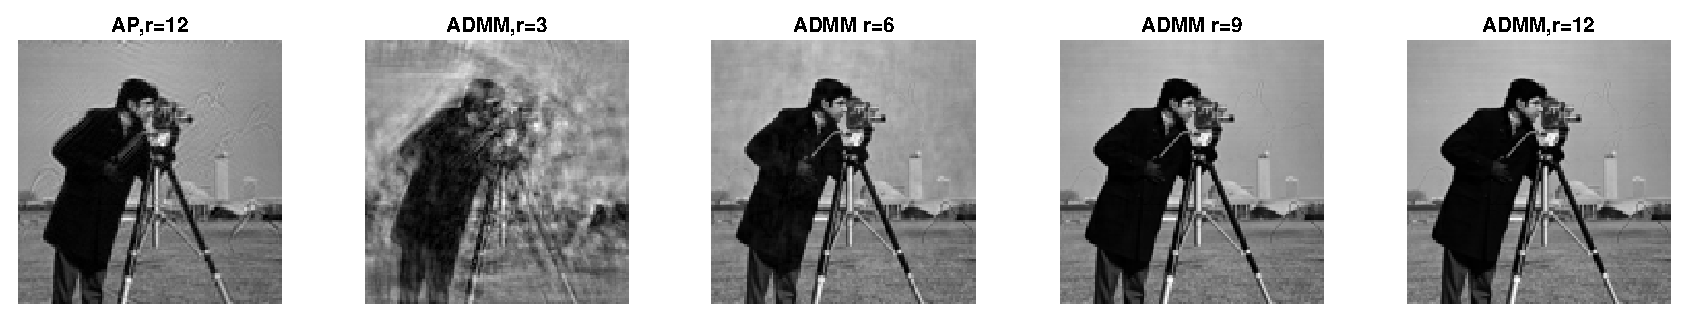
\includegraphics[width=0.9\linewidth]{../figures/modes_u.eps}  
		\caption{Amplitude}
		\label{fig:modes_u}
	\end{subfigure}
	\begin{subfigure}{1\textwidth}
		\centering
		% include second image
		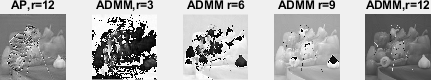
\includegraphics[width=.9\linewidth]{../figures/modes_u_phaze.png}  
		%\caption{Put your sub-caption here}
		\caption{Phase}
		\label{fig:modes_u_phaze}
	\end{subfigure}
	
	\label{fig:modes_images}
	\caption{Recovered images}
\end{figure}

\begin{figure}[H]
	\begin{subfigure}{.5\textwidth}
		\centering
		% include first image
		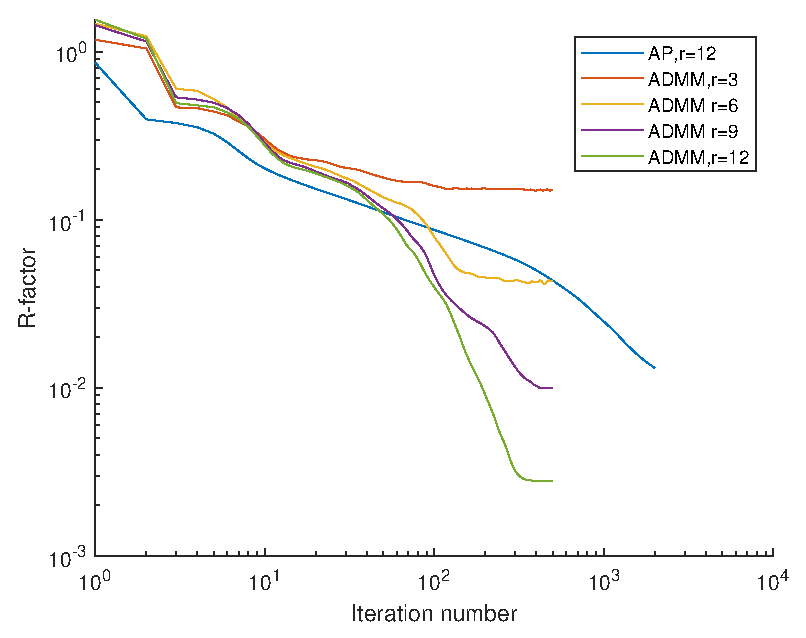
\includegraphics[width=0.9\linewidth]{../figures/modes_R.eps}  
		%\caption{}
		\label{fig:modes_R}
	\end{subfigure}
	\begin{subfigure}{.5\textwidth}
		\centering
		% include second image
		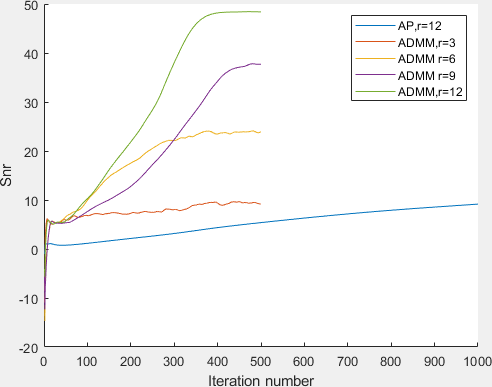
\includegraphics[width=.9\linewidth]{../figures/modes_snr.png}  
		%\caption{Put your sub-caption here}
		\label{fig:modes_snr}
	\end{subfigure}
	\caption{R and snr. }
	\label{fig:noise}
\end{figure}


%We first compare $snr$ and $R$ for reconstructed images using a different number of modes. When the number of modes increases, the $R-factor$ decreases, and the $snr$ increases. That indicates that the quality of the reconstructed image increases.
我们首先比较使用不同数量模态的重建图像的 $snr$ 和 $R$。 当模态数量增加时,$R-factor$ 减少,$snr$ 增加。 这表明重建图像的质量提高了。

使用 ADMM 算法的 3、6、9、12 个模态逼近算法时, $R$ 在 500 次迭代后稳定在 0.15、0.042、0.0099、0.0028,而 AP 的 $R$ 在 2000 次迭代后不收敛。


%fig2
\begin{figure}[H]
	\centering
	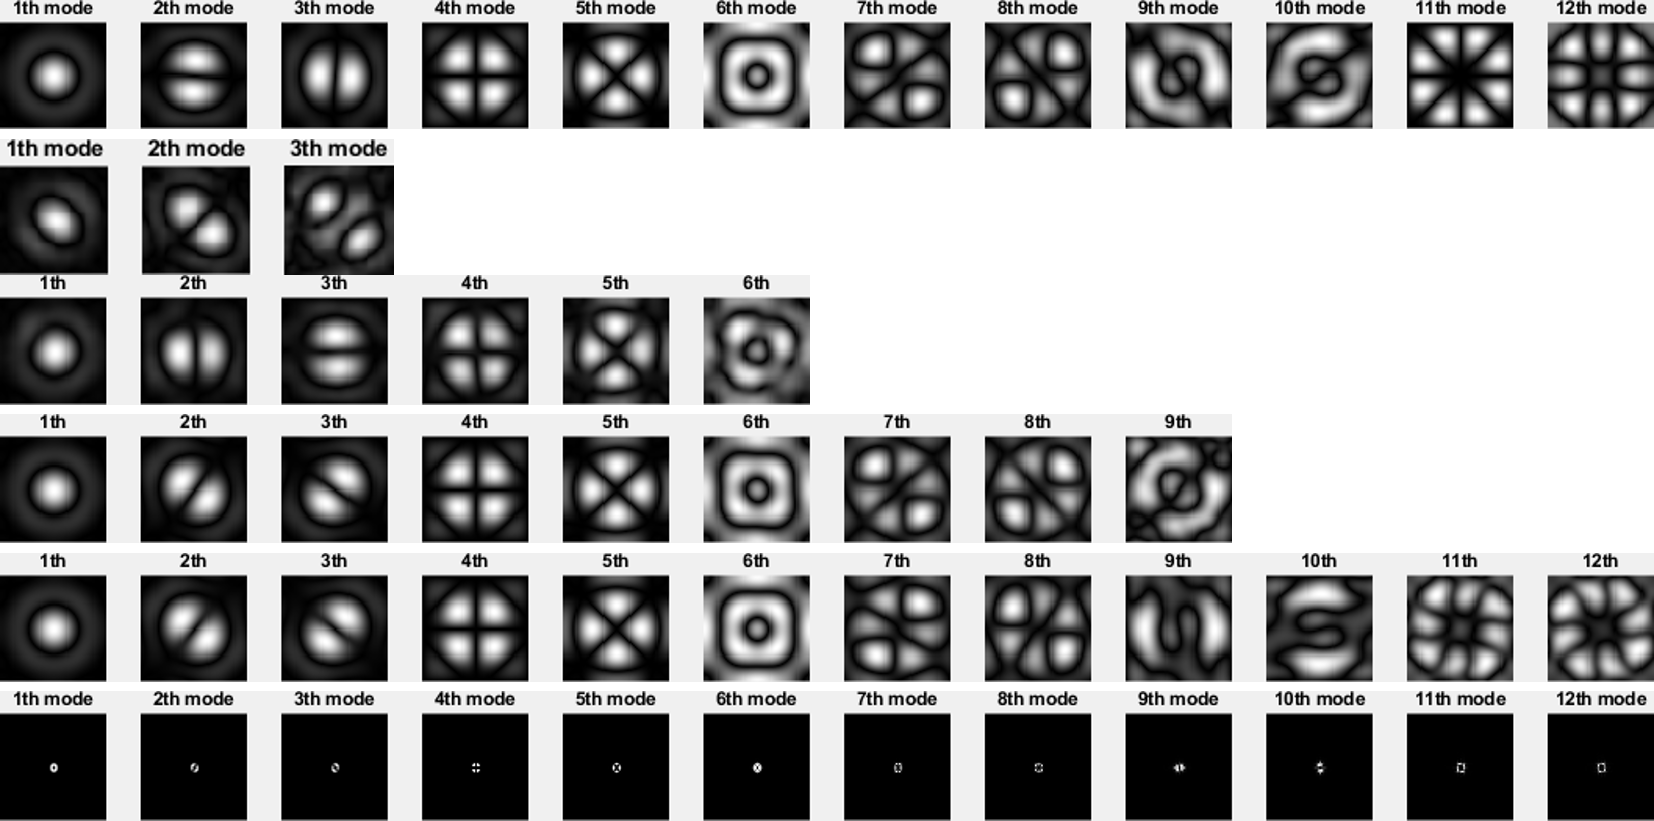
\includegraphics[width=1\linewidth]{../figures/modes_combine}
	\caption{%Mode pattern. The first row represents the standard mode pattern. And the last two rows represent the mode pattern for 12 modes. Mode patterns are in the time domain except that the last row is in the frequency domain.
	模态分解。 第一行代表“标准模态分解”。 最后两行代表 12 种模态的具体样式。 这里的模态被表示在在时域中,除了最后一行在频域中。}
	\label{fig:modescombine}
\end{figure}

%Standard mode pattern is obtained through performing SVD on standard density matrix generated from the model and extracting the first 12 modes. As shown in Figure \ref{fig:modescombine}, our algorithm can generally catch the main modes and get an optimal approximation.
“标准模态分解”是通过对模型生成的标准密度矩阵执行 SVD 并提取前 12 个模态获得的。 如图 \ref{fig:modescombine} 所示,我们的算法通常可以捕获主要模态并获得密度矩阵的最佳近似。

%fig3 
%Further, denote $err_M$ for r modes as $err_M^r$. Optimal $err_M^{r,*}$ can be calculated from the theory of low-rank approximation, and we compare our $err_M^r$ with it. Denote the singular values of standard density matrix $\rho_{true}$ as $s_i,i=1...d=rank(\rho_{true})$
此外,将 r 个模态的 $err_M$ 表示为 $err_M^r$。 最优 $err_M^{r,*}$ 可以从低秩逼近理论中计算出来,我们将我们的 $err_M^r$ 与它进行比较。 将标准密度矩阵 $\rho_{true}$ 的奇异值表示为

$$
err_M^{r,*} = \min_{\rho, rank(\rho)=r} \dfrac{||\rho_{true} - \rho||_F}{||\rho_{true}||_F} = \sqrt{\dfrac{\sum_{i=r+1}^{d}s_i^2}{\sum_i s_i^2}}
=
\sqrt{1 - s_{cum}(r)}
$$,
$$
where\ 
s_{cum}(r) = \dfrac{\sum_{i=1}^{r}s_i^2}{\sum_i s_i^2} 
$$

%fig 4 approx fig 
\begin{figure}
	\begin{subfigure}{.5\textwidth}
		\centering
		% include first image
		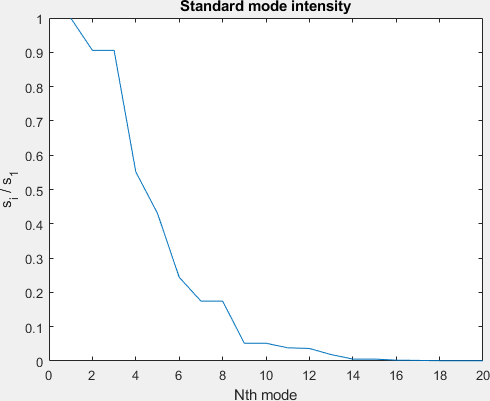
\includegraphics[width=0.9\linewidth]{../figures/singular.png}  
		%\caption{}
		\label{fig:singular}
	\end{subfigure}
	\begin{subfigure}{.5\textwidth}
		\centering
		% include second image
		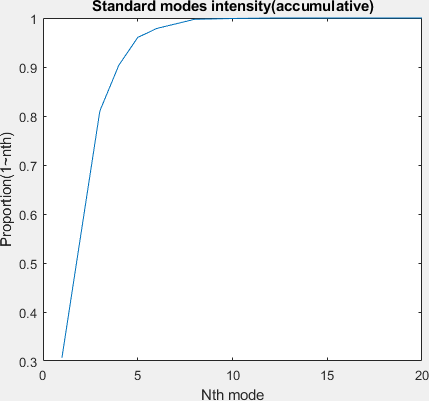
\includegraphics[width=.8\linewidth]{../figures/singular_accumative.png}  
		%\caption{Put your sub-caption here}
		\label{fig:singular_acc}
	\end{subfigure}
	\caption{标准密度矩阵的奇异值分布。 左边子图中的纵轴代表$i^{th}$最大奇异值与第一个$s_i/s_1$的比值,右边的纵轴代表$S_{cum}(i)$。 奇异值呈指数下降,矩阵近似低秩。 }
	\label{fig:standard singular}
\end{figure}

%As shown in Figure \ref{fig:approx error}, the $err_M^*$ reaches around $0.01$, and $err_M$ is close to $err_M^*$ with 12 modes, which indicates that our algorithm does well in low-rank approximation to standard density matrix.
如图 \ref{fig:approx error} 所示,$err_M^*$ 达到 $0.01$ 左右,$err_M$ 接近 $err_M^*$,有 12 种模态,这表明我们的算法在低秩逼近标准密度矩阵中做得不错。

\begin{figure}[H]
	\centering
	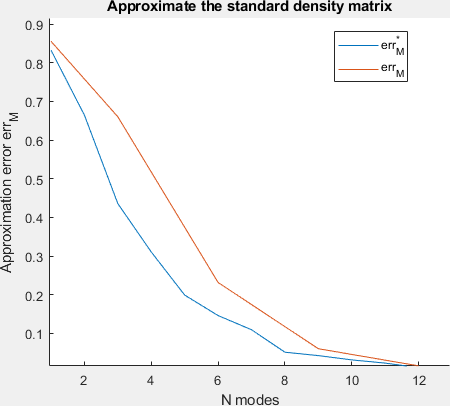
\includegraphics[width=0.8\linewidth]{../figures/approximation.png}
	\caption{}
	
	\label{fig:approx error}
	
\end{figure}

\subsection{实验二: 加入正交约束条件}
实验设置与上面相同,只是我们更改 $ratio=\beta_2/\beta$ 以在 ADMM 中引入正交化约束。 $\beta_2$ 越大,正交化约束越严格。 作为参考,我们还尝试按照算法 \ref{alg:ort} 每 20 次迭代对模态执行正交化操作。
%3
\begin{figure}[H]
	\begin{subfigure}{.33\textwidth}
		\centering
		% include first image
		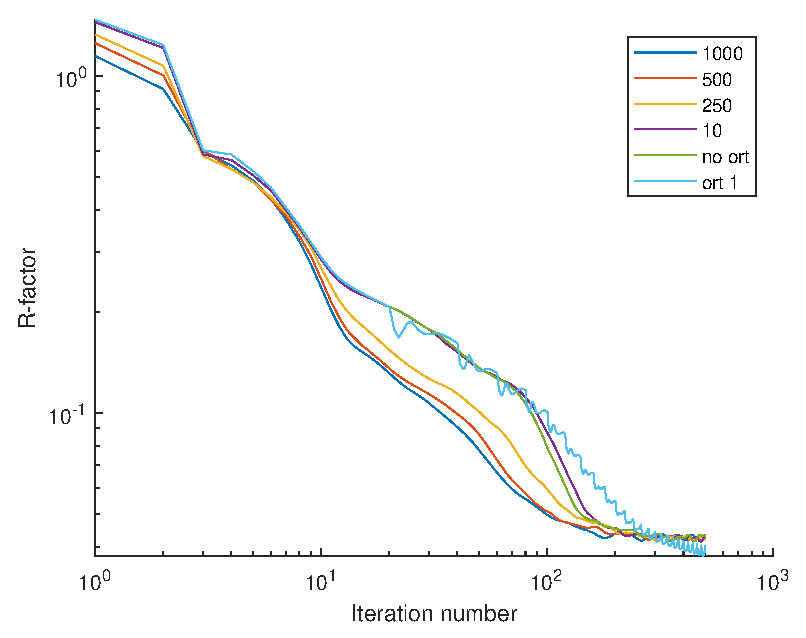
\includegraphics[width=1\linewidth]{../figures/ort_R.eps}  
		%\caption{}
		\label{fig:ort_R}
	\end{subfigure}
	\begin{subfigure}{.3\textwidth}
		\centering
		% include second image
		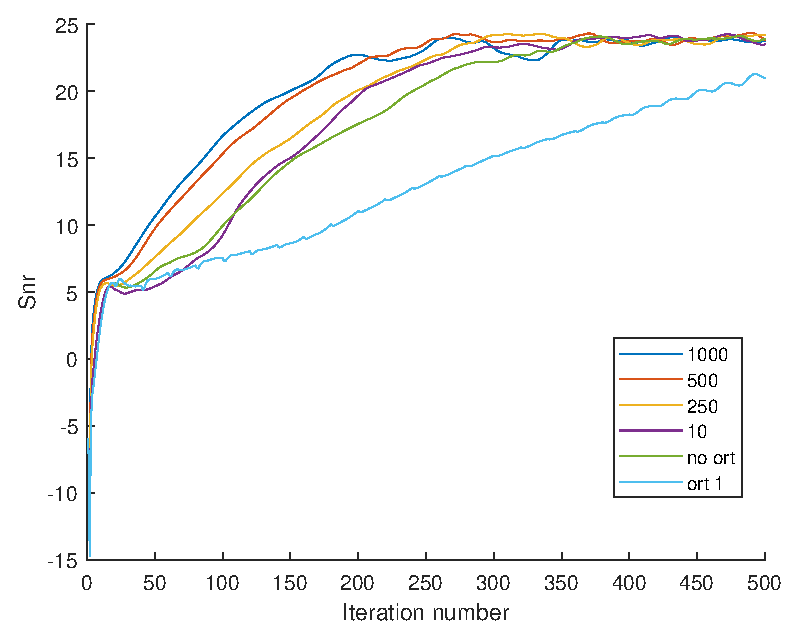
\includegraphics[width=1\linewidth]{../figures/ort_snr.eps}  
		%\caption{Put your sub-caption here}
		\label{fig:ort_snr}
	\end{subfigure}
	\begin{subfigure}{.3\textwidth}
		\centering
		% include second image
		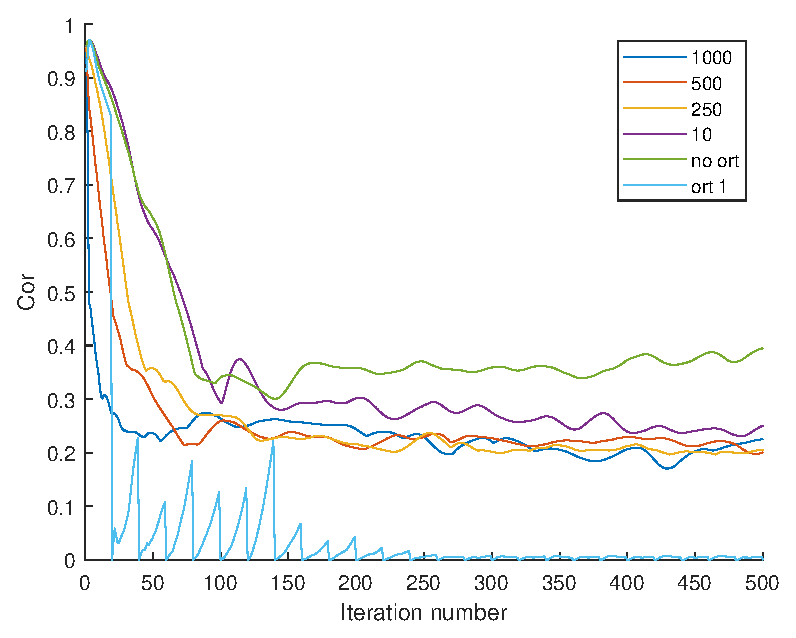
\includegraphics[width=1\linewidth]{../figures/ort_cor.eps}  
		%\caption{Put your sub-caption here}
		\label{fig:ort_cor}
	\end{subfigure}
	\caption{纵轴和横轴在 R 因子的第一个子图中以对数刻度设置。 蓝线代表 $\beta_2/\beta=1000$,在这种情况下效果最好。 绿线表示没有正交化的结果。 “ort 1”表示每 20 次迭代执行一次正交化。 }
	\label{fig:ort}
\end{figure}
500次迭代后重建的图像相似,而使用具有正交化约束的 ADMM 算法的 $snr$ 和 $R factor$ 改进更快。 并且随着 $\beta_2$ 的增大,模态之间的相关度 $coherence$ 也会下降得更快。



%%\noindent\textbf{Remark.}

%1. We suppose that orthogonalization constraints can improve robustness on different initial values. 

%2. When the number of modes is large enough(like 12 here), the effect of the orthogonalization constraint seems not noticeable.

\subsection{实验三:有噪声的情形}
$Dist=8$, $gridFlag=3$, $blurFlag=2$ 和 $\kappa$ 是一个高斯核,$\sigma = (15,15)$, $\beta=0.05$。

通过 MATLAB 命令在衍射图像 $Y$ 上添加泊松噪声:
$$
Y_{噪声}=poissrnd(Y*(\eta))/\eta;
$$

这里使用 $\eta=0.0675$。

%Four different settings are compared: 9 modes with noise, 9 modes with noise, and 6 are kept after compression, 6 modes with noise, and 6 modes without noise(standard). Specifically, we conducted compression as in \ref{alg:compression} every 20 iterations, and kept 6 modes each time.
比较了四种不同的设置:9 个模态带噪声、9 个模态无噪声、6个模态在压缩操作之后被保留、6 个模态带噪声和 6 个模态无噪声。 具体来说,我们按照 \ref{alg:compression} 每 20 次迭代进行压缩,每次保持 6 个模态。
%fig6 differet setting images, R, (snr without st)

\begin{figure}
	\centering
	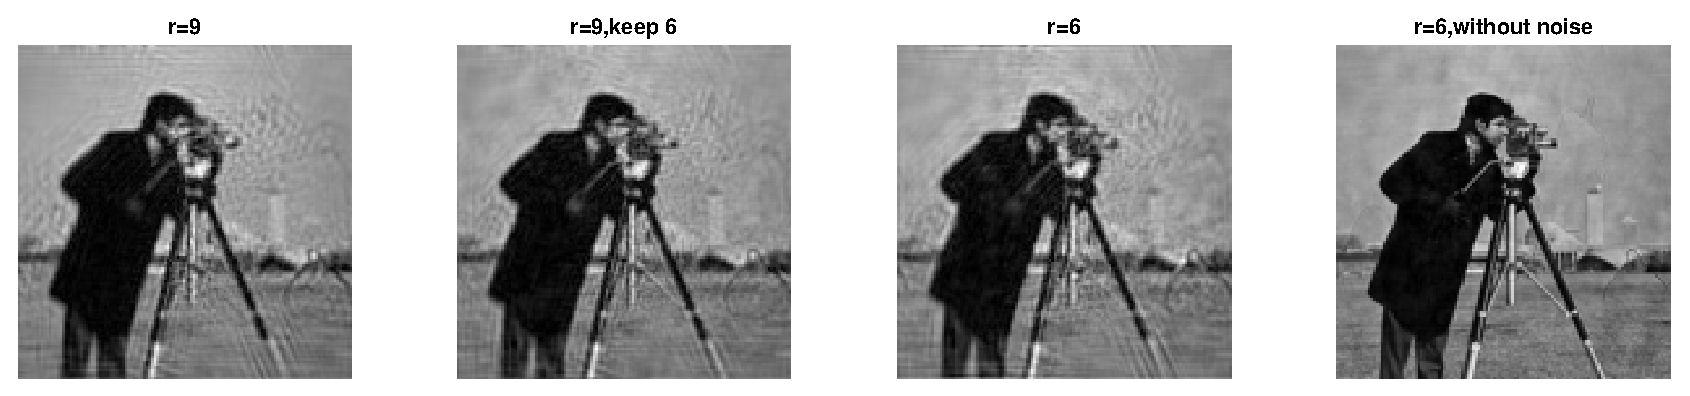
\includegraphics[width=1\linewidth]{../figures/noise_u.eps}
	\caption{Reconstructed images in the noisy case}
	
	\label{fig:noise_u}
	
\end{figure}

\begin{figure}
	\begin{subfigure}{.5\textwidth}
		\centering
		% include first image
		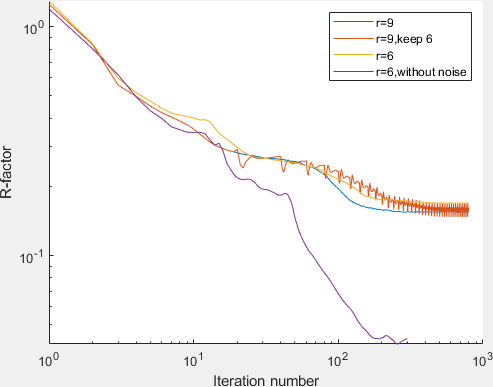
\includegraphics[width=0.9\linewidth]{../figures/noise_R.png}  
		%\caption{}
		\label{fig:noise_R}
	\end{subfigure}
	\begin{subfigure}{.5\textwidth}
		\centering
		% include second image
		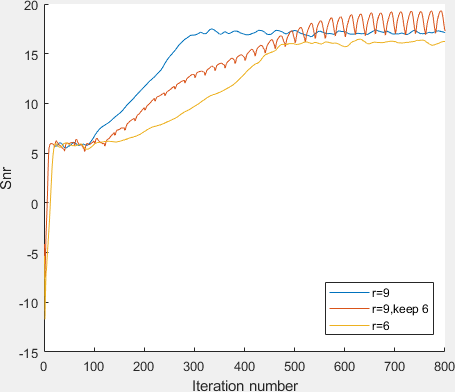
\includegraphics[width=.8\linewidth]{../figures/noise_snr.png}  
		%\caption{Put your sub-caption here}
		\label{fig:noise_snr}
	\end{subfigure}
	\caption{R and snr. The red line represents the result with compression.}
	\label{fig:noise}
\end{figure}

结果随着压缩操作周期性地波动,而最终在嘈杂的情况下表现最好。 虽然差异并不明显,但这个现象引导我们思考,未来我们或许可以以考虑在ADMM的约束中添加压缩,而不是执行直接截断操作,将压缩操作和ADMM算法融合。

\section{总结和展望}

在本文中, 我们选择了“探针振动模型”(\ref{model:gradient decomposition}) 刻画偏相干效应,作为目标模型。 经过对不同模型的详细讨论, 具体刻画了目标模型密度矩阵的特殊结构, 将它放入通用模型的框架中。

然后,改进了求解通用模型的相位恢复算法。 第一,将多模态AP改进为多模态的ADMM。 第二,尝试在里面加入对不同模态的正交约束。

最后,用模型生成仿真数据,完成了三个数值实验,并与传统AP的计算结果和基于模型得到的“标准答案”进行对比,验证的算法的有效性。

虽然我们说明了,将目标模型放入通用模型框架下求解合理而且有效,但是没有利用到里面的特殊结构十分可惜。 通用模型可以求解任何近似$rank-r$的密度矩阵,而我们目标模型中的密度矩阵结构更特殊: 一个toeplitz矩阵与一个秩一矩阵逐个元素相乘。 如何分解、近似这种特殊结构的矩阵,是未来工作的重要方向。

\newpage 
\section{附录}
\subsection{ADMM中的子问题}
\label{section:subproblems}
\subsubsection{$\omega$}
本质上,在这个子问题中,每个状态 $\omega_i=w(:,:,i)$ 都是独立的。 然后我们可以分别优化每个$w_i$。
$$
\omega_i^{k+1}=\arg \min _{\omega \in \mathcal{X}_{1}} \frac{1}{2} \sum_{j}\left\|\mathcal{F}^{-1} \hat{z}(:,:,j,i)^{k}-\omega(:,:,i) \circ \mathcal{S}_{j} u^{k}\right\|^{2}
$$

本质上,在这个子子问题中,$w_i$ 中的每个元素都是独立的。
这样只需要解决以下一维约束二次问题:
$$
\omega_i^{k+1}(t)=\arg \min _{|x| \leq C_{\omega}} \rho_{t}^{k}(x).
$$
这里
$\rho_{t}^{k}(x):=\frac{1}{2} \sum_{j}\left|\left(\mathcal{F}^{-1} \hat{z}(:,:,j,i)^{k}\right)(t)-x \times\left(\mathcal{S}_{j} u^{k}\right)(t)\right|^{2} \forall x \in \mathbb{C}$ 

计算$\rho_{t}^{k}(x)$的导数。注意这里$\rho$ 是一个复变量实值函数,我们使用wirtinger 导数。 
$$
\begin{aligned}
&\nabla \rho_{t}^{k}(x) = \dfrac{ d\rho_{t}^{k}(x)}{dx^*} \\
&\begin{aligned}
=\sum_{j}\left(x \times\left|\left(\mathcal{S}_{j} u^{k}\right)(t)\right|^{2}-\left(\mathcal{S}_{j} u^{k}\right)^{*}(t)\left(\mathcal{F}^{-1} \hat{z}_{j,i}^{k}\right)(t)\right)
\end{aligned} \\
&\begin{aligned}
=x \times\left(\sum_{j}\left|\left(\mathcal{S}_{j} u^{k}\right)(t)\right|^{2}\right)-\sum_{j}\left(\left(\mathcal{S}_{j} u^{k}\right)^{*}(t)\left(\mathcal{F}^{-1} \hat{z}_{j,i}^{k}\right)(t)\right) \\
\end{aligned}
\end{aligned}
$$
一阶最优条件是$\nabla \rho_{t}^{k}(x)=0 $。 然后 $w_i$ 的闭形式解给出为
$$
\omega_i^{k+1}=\operatorname{Proj}\left(\frac{ \sum_{j}\left(\mathcal{S}_{j} u^{k}\right)^{*} \circ\left(\mathcal{F}^{-1} \hat{z}_{j,i}^{k}\right)}{ \sum_{j}\left|\mathcal{S}_{j} u^{k}\right|^{2}} ; C_{\omega}\right)
$$

\subsubsection{z}
$$
\quad z^{k+1}=\arg \min _{z} \mathcal{G}(z)+\frac{\beta}{2}\left\|z-\mathcal{A}\left(\omega^{k+1}, u^{k+1}\right)+\Lambda^{k}\right\|^{2}\\
$$
$$
=\arg \min _{z} \frac{1}{2}|| \sqrt{ \sum_{i=1}^{r} |z(:,:,:,i)|^2} - Y||^2+\frac{\beta}{2}\left\|z - z^+\right\|^{2}
$$
$$
= \arg \min _{z} \sum_{x,y,j} [\frac{1}{2} ( \sqrt{ \sum_{i=1}^{r} |z(x,y,j,i)|^2} - Y(x,y,j) )^2 +
\frac{\beta}{2}||z(x,y,j,:) - z^+(x,y,j,:)||^2 ]
$$

这里 $z^+ = \mathcal{A}\left(\omega^{k+1}, u^{k+1}\right) - \Lambda^{k}$

对于任意固定的$x,y,j$和自由的$i$,问题可以看成:

$$
z^*(x,y,j,:) = \arg \min_{z_{x,y,j} \in \mathbb{C}^{r}} \frac{1}{2} ( ||z_{x,y,j}|| - Y_{x,y,j} )^2
+ \frac{\beta}{2} ||z_{x,y,j} - z_{x,y,j}^+||^2
$$

请注意,对于固定的 $||z_{x,y,j}||$,表达式中的第一项是固定的。 为了优化第二项,我们应该始终选择与 $z_{x,y,j}^+$ 方向相同的 $z_{x,y,j}$。 所以我们有 $||z_{x,y,j} - z_{x,y,j}^+||^2 = (||z_{x,y,j}|| - ||z_{x, y,j}^+||)^2$
$$
\dfrac{z(x,y,j,i)}{||z_{x,y,j}||} = \dfrac{z^+(x,y,j,i)}{||z_{x,y,j}^+||}, z(x,y,j,i) = ||z_{x,y,j}||\dfrac{z^+(x,y,j,i)}{||z_{x,y,j}^+||}
$$
要确定$z_{x,y,j}$,我们只需要确定$||z_{x,y,j}||$。 将其表示为$a$。
$$
||z_{x,y,j}||^* = \arg \min_{a \in \mathbb{R}} \frac{1}{2}(a - Y_{x,y,j})^2 + \dfrac{\beta}{2}
(a - ||z_{x,y,j}^+||)^2
$$
一阶最优性条件很容易给出:
$$
a = \dfrac{Y_{x,y,j} + \beta ||z_{x,y,j}^+||}{1 + \beta}
$$
步骤 3 的闭式形式解为:

\begin{equation}
z_i^{k+1} = \dfrac{z^+ \dfrac{Y}{ M^k} + \beta z_i^+}{1+\beta}, 1 \leq i \leq r
\label{zup}
\end{equation}
where $M^k =\sqrt{\sum_i |z^+(:,:,:,i)|^2} \in \mathbb{C}^{px \times py \times N}$

\subsubsection{D}

$$
\begin{aligned}
D^{k+1} =& \arg \min_{D} \| \Omega -  w^{k+1} + \Lambda_2^{k}\|^{2} \\
=& \arg \min_{D} \| D\alpha^k - \hat {w}^{k+1}\|^{2} 
\end{aligned}
$$
where $\hat {w}^{k+1} = reshape( \omega^{k+1} - \Lambda_2^{k},[px\times py,r])$,$D^*D=I$

这是正交 Procrustes 问题中的一个特例. \footnote{\url{https://en.wikipedia.org/wiki/Orthogonal_Procrustes_problem}}
$$
\begin{aligned}
\| D\alpha^k - \hat {w}^{k+1}\|^{2} =& Tr[( D\alpha^k - \hat {w}^{k+1})^*( D\alpha^k - \hat {w}^{k+1})] \\
=& ||\alpha^k||_F^2 - Tr[(\alpha^k)^*D^*\hat{\omega}^{k+1}] - Tr[(\hat{\omega}^{k+1})^*D \alpha^k] + ||\hat{\omega}^{k+1}||_F^2
\end{aligned}
$$
$$
\begin{aligned}
D^{k+1} =& \arg \max_{D} Tr[(\alpha^k)^*D^*\hat{\omega}^{k+1}] + Tr[(\hat{\omega}^{k+1})^*D \alpha^k] \\
=& \arg \max_{D}  \Re{ (Tr[(\alpha^k)^*D^*\hat{\omega}^{k+1}] )}\\
\xlongequal{\alpha \in \mathbb{R}^{r\times r}}& \arg \max_{D}  \Re{ (Tr[D^* ( \hat{\omega}^{k+1}\alpha^k)]  )}
\end{aligned}
$$
考虑 SVD 分解: $\hat{\omega}^{k+1}\alpha^k = USV^*$
$$
\begin{aligned}
D^{k+1} &= \arg \max_{D} \Re{ (Tr[D^*USV^*]  )}
= \arg \max_{D} \Re{ (Tr[(V^*D^*U)S]  )}\\
&\xlongequal{\hat{D} = V^*D^*U}  \arg \max_{\hat{D}} \Re{ (Tr[\hat{D}S]  )}
\end{aligned}
$$
我们得到 $\hat{D} = I_r$时是最优的, $I_r$为前$r$个对角元为1,其余为0的对角阵。 而且:
\begin{equation}
D^{k+1} = UV^*
\label{Dup}
\end{equation}

\section{致谢}
四年的时间转眼而过。 怀着忐忑的心情转专业来到数学学院, 在这里收获了很多,也找到了自己喜欢的东西。

感谢家人对我无条件的支持,妈妈一个人把我养到那么大实属不易,我一直被保护得很好。

感谢数院老师一路上的指导和帮助。 杨力华老师精彩的数值分析课在我心中留下一颗种子,老师很耐心地告诉我计算数学的几大方向,让我对未来感到清晰许多。 李嘉老师讲的数学实验与数学软件也十分精彩,让我相信了计算和应用数学的力量, 这颗种子最终生根发芽, 成为我博士研究生的方向。

感谢天津师范大学数学学院的常慧宾老师提供了这个有趣的毕业课题, 并耐心地给予我指导。 计算光学是一个很有趣的方向,希望能把这个问题研究得更深入,做出好的成果。

很幸运拥有温暖的舍友们,矩阵分析刷题小组的兄弟们, 排球队的姐姐妹妹们,还有许多许多可爱的人们。 

我会永远记住这段美好的时光,在我最青春的大学四年中,和好朋友一起学习数学知识,一起做题,并且有幸遇到这么多好的老师和同学们,每个积极向上,热情洋溢的日子都是如此的美好。

\newpage
	\bibliographystyle{unsrtnat}
 \bibliography{wt}
 

	
	
	
	

	

	
	
	
	
	
\end{document}





